\section{Component Diagram cho Task Assignment Module}
    \subsection{Component Diagram Task Assignment}
         \begin{figure}[h]
            \centering
            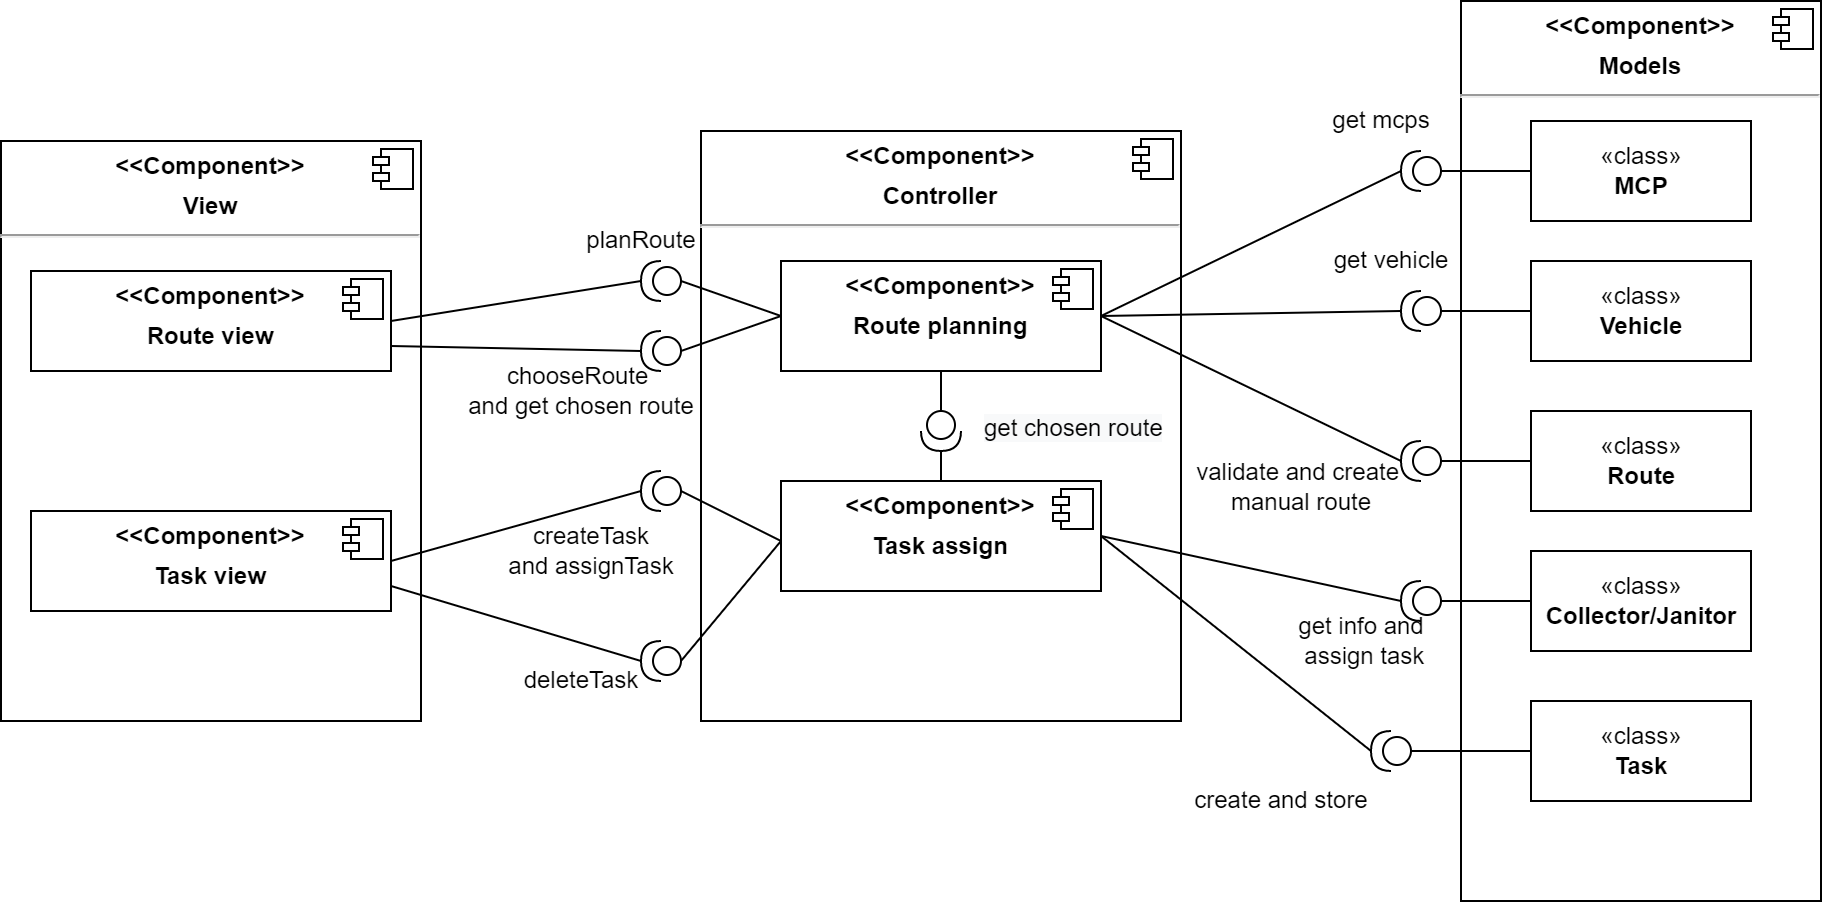
\includegraphics[width=1\linewidth]{imgs/component diagram/component Task Assignment.png}
            \caption{Component diagram cho task assignment module}
        \end{figure}
        Component diagram Task Asignment module gồm 5 Component với luồng thực thi:
        \begin{enumerate}
            \item Đưa dữ liệu Vehicle và MCPs vào Component Planning route và trả về tuyến đường khả dụng.
            \item Đưa dữ liệu các tuyến đường khả dụng vào component Choose route và trả về tuyến đường đã được Back Officer chọn.
            \item Đưa tuyến đường được chọn và Task vào Component Assign route, dữ liệu trả về là Task đã được Assign route.
            \item Đưa dữ liệu Task đã được Assign vào component Schedule time và trả về dữ liệu là Task được định thời gian thực hiện.
            \item Đưa lịch làm đã xếp và Worker vào component Assign staff và trả về kết quả là Task đã được Assign Worker, vehicle, route, calendar. 
        \end{enumerate}
    \subsection{Component Diagram cho Planning Route }
        \begin{figure}[h]
            \centering
            \includegraphics[width=1\linewidth]{imgs/Component diagram/Component planning route.png}
            \caption{Component diagram cho Planning Route}
        \end{figure}
        Component diagram cho Planning Route gồm 2 Component thừa kế Component Modification Method với luồn thực thi:
        \begin{itemize}
            \item Auto generate route:
            \begin{enumerate}
                \item Đưa dữ liệu Vehicle, MCPs vào Component Get Avaiable Paths và trả về tuyến đường khả thi.
                \item Đưa dữ liệu các tuyến đường khả dụng vào Component Generate routes and Efficiency Statistic và trả về kết quả là tuyến đường hiệu quả để sử dụng.
            \end{enumerate}

            \item Manual generate route:
            \begin{enumerate}
                \item Đưa dữ liệu tuyến đường vào Component Validate Routes để kiểm thử và trả về tuyến đường đã được kiểm tra.
                \item Đưa tuyến đường đã được kiểm tra vào Component Generate routes and Efficiency Statistic và trả về kết quả là tuyến đường hiệu quả để sử dụng.
            \end{enumerate}
        \end{itemize}
        
       